% !TEX TS-program = pdflatex
% !TEX encoding = UTF-8 Unicode

% This is a simple template for a LaTeX document using the "article" class.
% See "book", "report", "letter" for other types of document.

\documentclass[11pt]{paper} % use larger type; default would be 10pt

%%% Examples of Article customizations
% These packages are optional, depending whether you want the features they provide.
% See the LaTeX Companion or other references for full information.

%%% PAGE DIMENSIONS
%\usepackage{geometry} % to change the page dimensions
%\geometry{a4paper} % or letterpaper (US) or a5paper or....
% \geometry{margin=2in} % for example, change the margins to 2 inches all round
% \geometry{landscape} % set up the page for landscape
%   read geometry.pdf for detailed page layout information
\usepackage{mathtools}
\usepackage{graphicx} % support the \includegraphics command and options

% \usepackage[parfill]{parskip} % Activate to begin paragraphs with an empty line rather than an indent

%%% PACKAGES
%\usepackage{booktabs} % for much better looking tables
%\usepackage{array} % for better arrays (eg matrices) in maths
%\usepackage{paralist} % very flexible & customisable lists (eg. enumerate/itemize, etc.)
%\usepackage{verbatim} % adds environment for commenting out blocks of text & for better verbatim
%\usepackage{subfig} % make it possible to include more than one captioned figure/table in a single float
% These packages are all incorporated in the memoir class to one degree or another...

%%% HEADERS & FOOTERS
%\usepackage{fancyhdr} % This should be set AFTER setting up the page geometry
%\pagestyle{fancy} % options: empty , plain , fancy
%\renewcommand{\headrulewidth}{0pt} % customise the layout...
%\lhead{}\chead{}\rhead{}
%\lfoot{}\cfoot{\thepage}\rfoot{}

%%% SECTION TITLE APPEARANCE
%\usepackage{sectsty}
%\allsectionsfont{\sffamily\mdseries\upshape} % (See the fntguide.pdf for font help)
% (This matches ConTeXt defaults)

%%% ToC (table of contents) APPEARANCE
%\usepackage[nottoc,notlof,notlot]{tocbibind} % Put the bibliography in the ToC
%\usepackage[titles,subfigure]{tocloft} % Alter the style of the Table of Contents
%\renewcommand{\cftsecfont}{\rmfamily\mdseries\upshape}
%\renewcommand{\cftsecpagefont}{\rmfamily\mdseries\upshape} % No bold!

%%% END Article customizations

%%% The "real" document content comes below...

\title{Infering the volume of binding pocket of odor-receptors in Drosophila from the neural data}
\author{Majid Saberi \and Hamed Seyed-allaei\thanks{hamed@ipm.ir}}
\institution{School of Cognitive Science, Institute for Research in Fundamental Sciences (IPM), \\Tehran, Iran}
%\date{} % Activate to display a given date or no date (if empty),
         % otherwise the current date is printed 


\begin{document}
\maketitle
\begin{abstract}
To be writen later.
\end{abstract}

\section{Introduction}

odor receptors.

\section{Methods}

Let the response of receptor neuron $n$ to the molecule $m$ be $r_{nm}$. 
The response $r_{nm}$ depends on the volume of the molecule, $v_m$, 
and many other physio-chemical properties of the molecule $m$.
Therefore, we separate the response $r_{nm}$ in two terms, 
\begin{equation}
r_{nm} = f_n(v_m) \psi_{nm}.
\label{eqn:factors}
\end{equation}
The first term, $f_n(v)$, depends only on the molecular volume of odorants.
The second term, $\psi_{nm}$ may include every other properties of molecules, but the molecular volume.
Both terms are characteristic of each receptor, and they might vary from neuron to neuron.
In fact, the first term, $f_n(v)$, is the tuning curve of neuron $n$ in respect to the feature of molecular volume, 
and like many other tuning curves, it can be approximated with a Gaussian function
\[
\displaystyle f_n(v) = e^{-\frac{(v-v_n)^2}{2\sigma^2_n}}, 
\]
where, $v_n$ is the preferred molecular volume of receptor $n$ and $\sigma_n$ represents its volume selectivity. 
In this work we want to estimate $v_n$ and $\sigma_n$. 
To do so, first we calculate the response weighted average of molecular volumes, 
$\frac{\sum_m v_m r_{nm}}{\sum_m r_{nm}}$ and then we use equation \ref{eqn:factors} to expand it:
\[
\frac{\displaystyle \sum_m v_m r_{nm}}{\displaystyle \sum_m r_{nm}} = \frac{\displaystyle \sum_m v_m f_n(v_m) \psi_{nm}}{\displaystyle \sum_m f_n(v_m) \psi_{nm}}.
\]
Here we can replace $\sum_m$ with $\int dv$:
\[
\sum_m \dots f_n(v_m) \psi_{nm} =  \langle \psi_{nm} \rangle_m \int_0^\infty \dots f_n(v) g(v)  dv, 
\]
in which, $\langle \psi_{nm} \rangle_m$ denotes the average of $\psi_{nm}$ over variable $m$, 
and $g(v)$ is the density of states, it says the molecular volume of how many odorants are between $v$ and $v+dv$.
The density of states, $g(v)$, is a characteristic of odorants and it can be approximated with a Gaussian function as well, 
\[
\displaystyle g(v) = e^{-\frac{(v- \langle v_m \rangle)^2}{2\sigma_{v}^2}},
\]


\[
h_n(v) = f_n(v) g(v)
\]


\[
\sum_m \dots f_n(v_m) \psi_{nm} = \langle \psi_{nm} \rangle_m \int_v \dots h_n(v) dv 
\]



\[
\displaystyle h(v) = e^{-\frac{(v-\mu_n)^2}{2\sigma^2}}
\]


\begin{eqnarray}
\frac{\sum_m v_m r_{nm}}{\sum_m r_{nm}} &=& \frac{\langle \psi_{nm} \rangle_m \int_v v h_n(v) dv }{\langle \psi_{nm} \rangle_m \int_v  h_n(v) dv }\\
 &=& \frac{\int_v v h_n(v) dv}{ \int_v  h_n(v) dv } \\
 &=& \langle v \rangle_{h_n}
\end{eqnarray}•


gaussian dists, source of data, etc.

\section{Results}

\begin{enumerate}
\item Volumes + errors.
\item Std of volumes + errors.
\end{enumerate}•

\begin{figure}
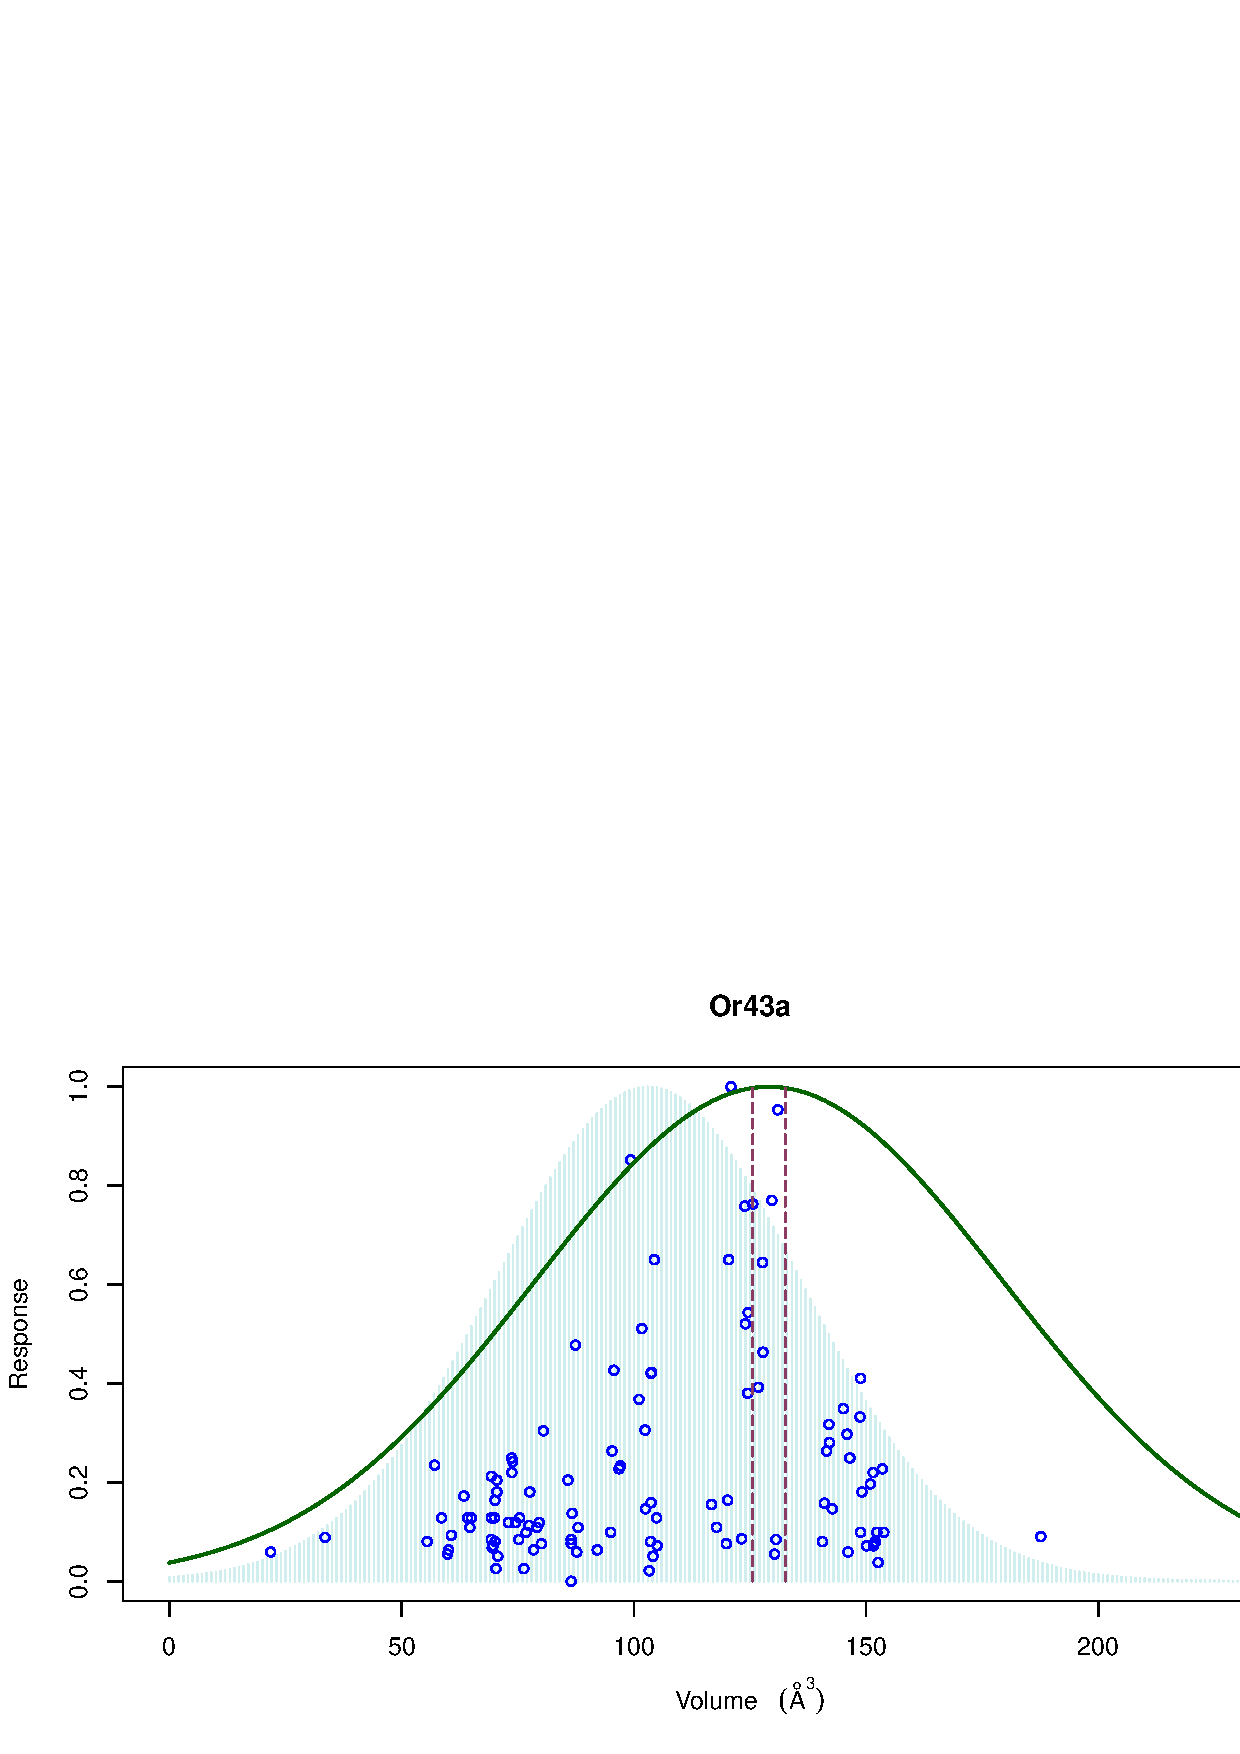
\includegraphics[width=\textwidth]{fig/vol-res-Or42a}
\caption{Response of an odor-receptor (Or42a) versus molecular volume of odorants.}
\end{figure}•

\begin{figure}
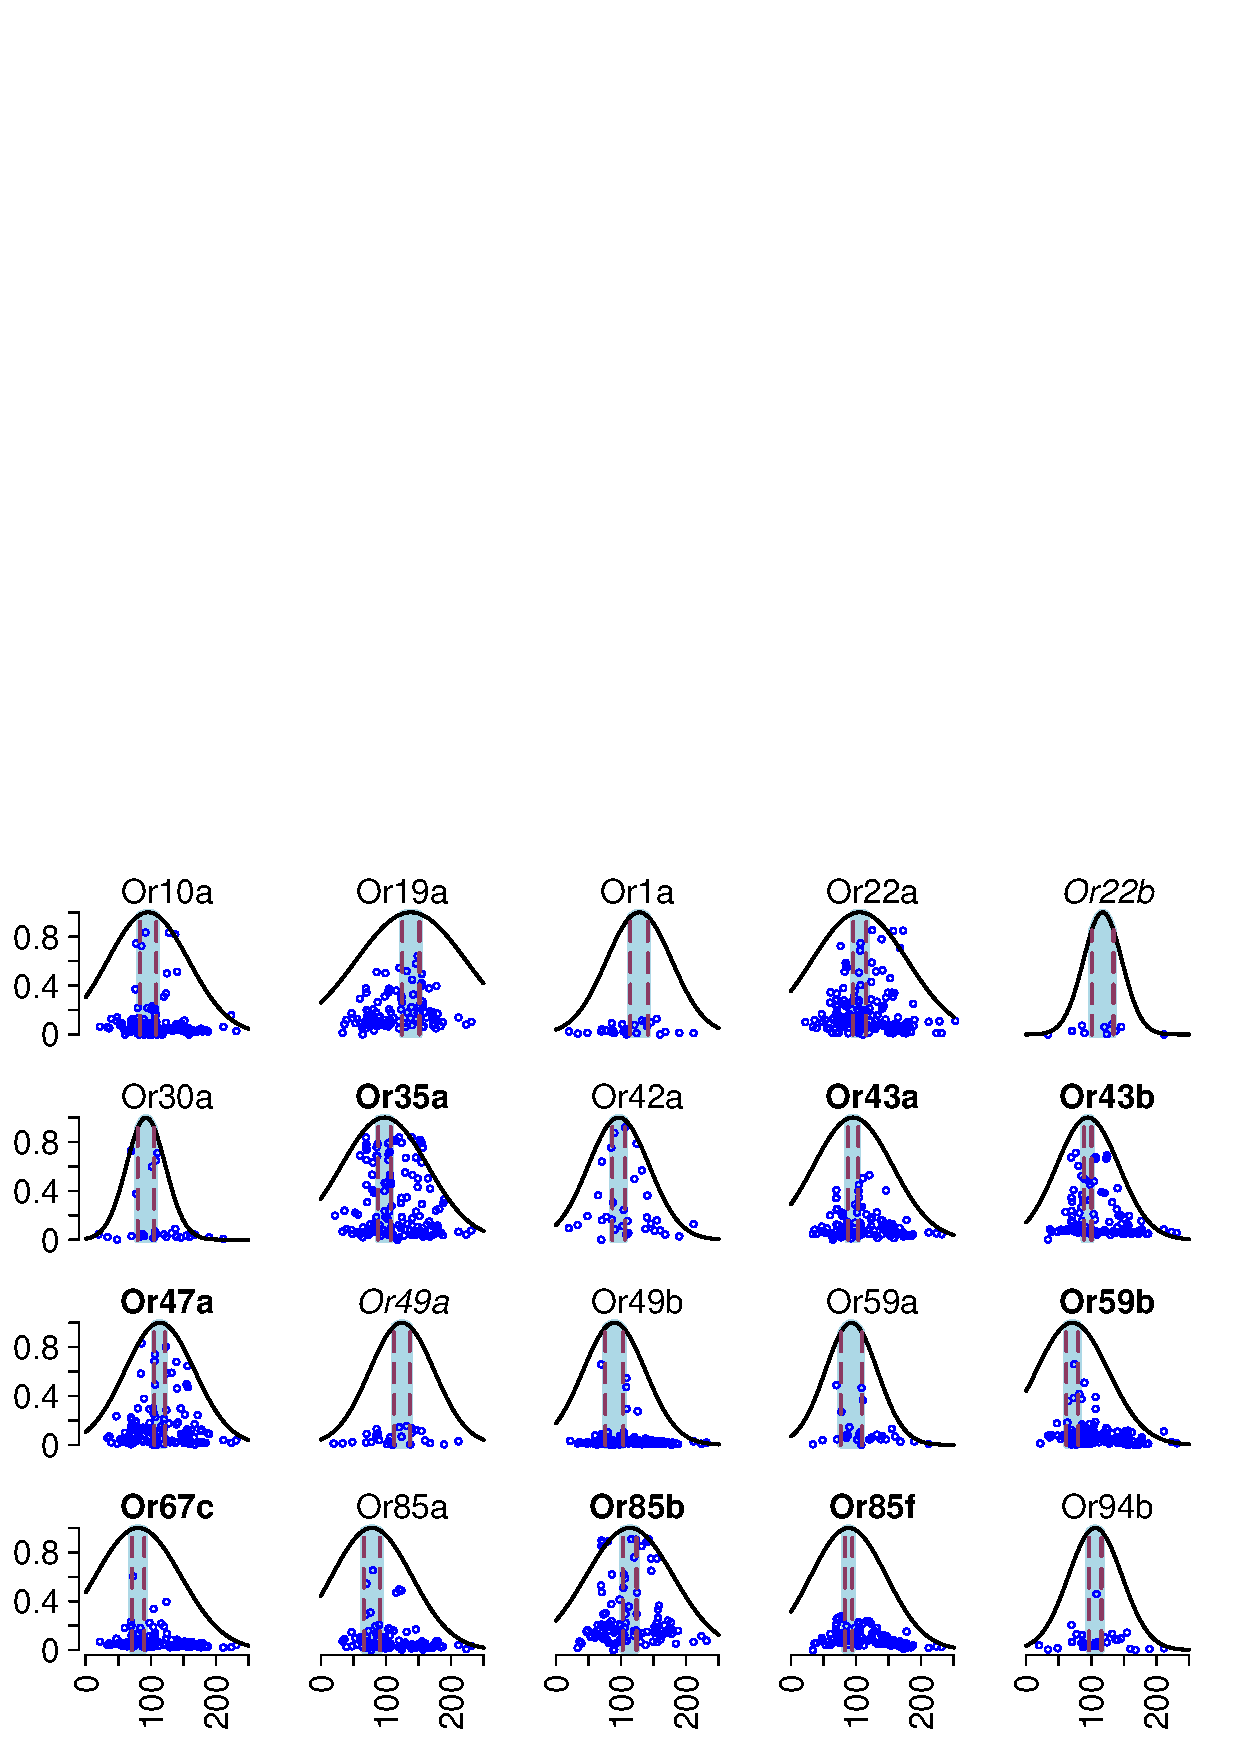
\includegraphics[width=\textwidth]{fig/vol-res}
\caption{Response of odor-receptors  versus molecular volume of odorants.}
\end{figure}•

\begin{figure}
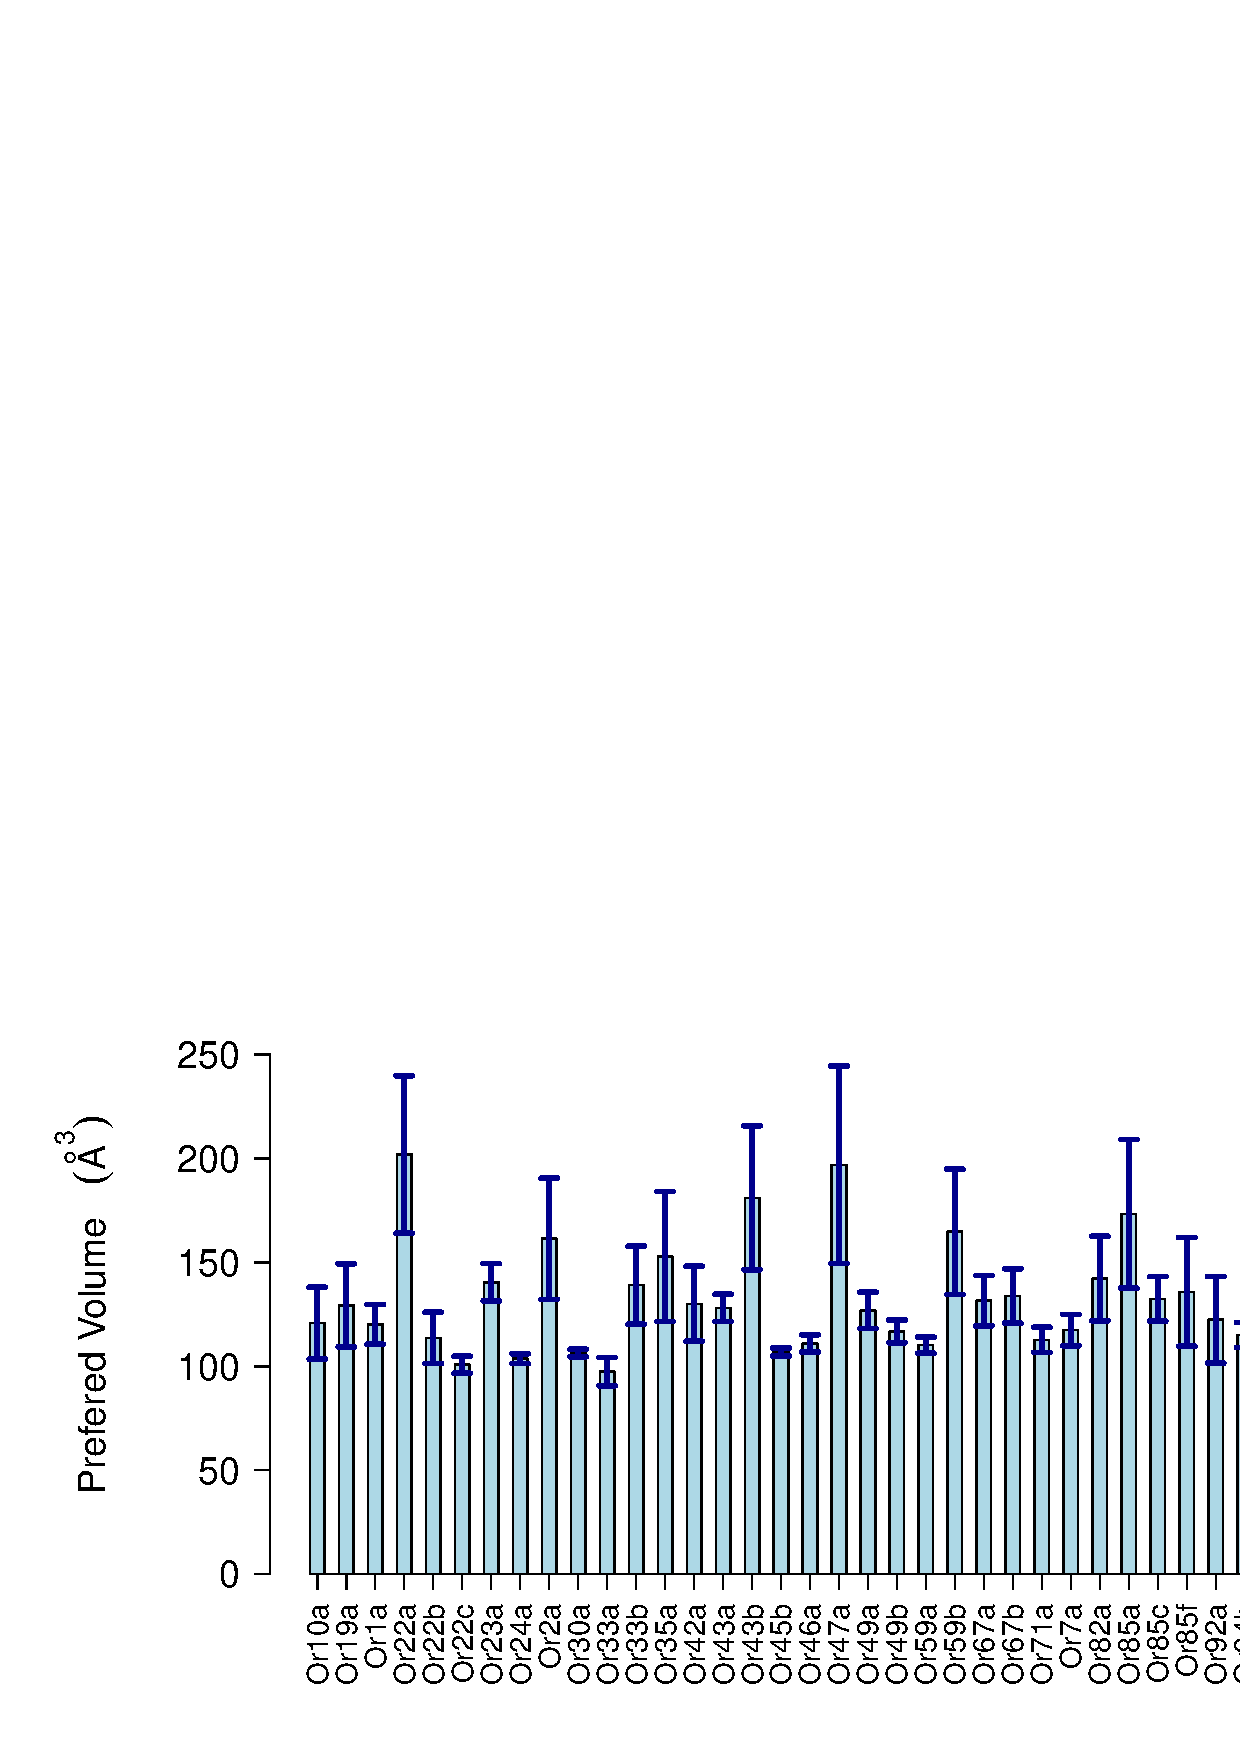
\includegraphics[width=\textwidth]{fig/mean-vol}
\caption{mean volume.}
\end{figure}•

\begin{figure}
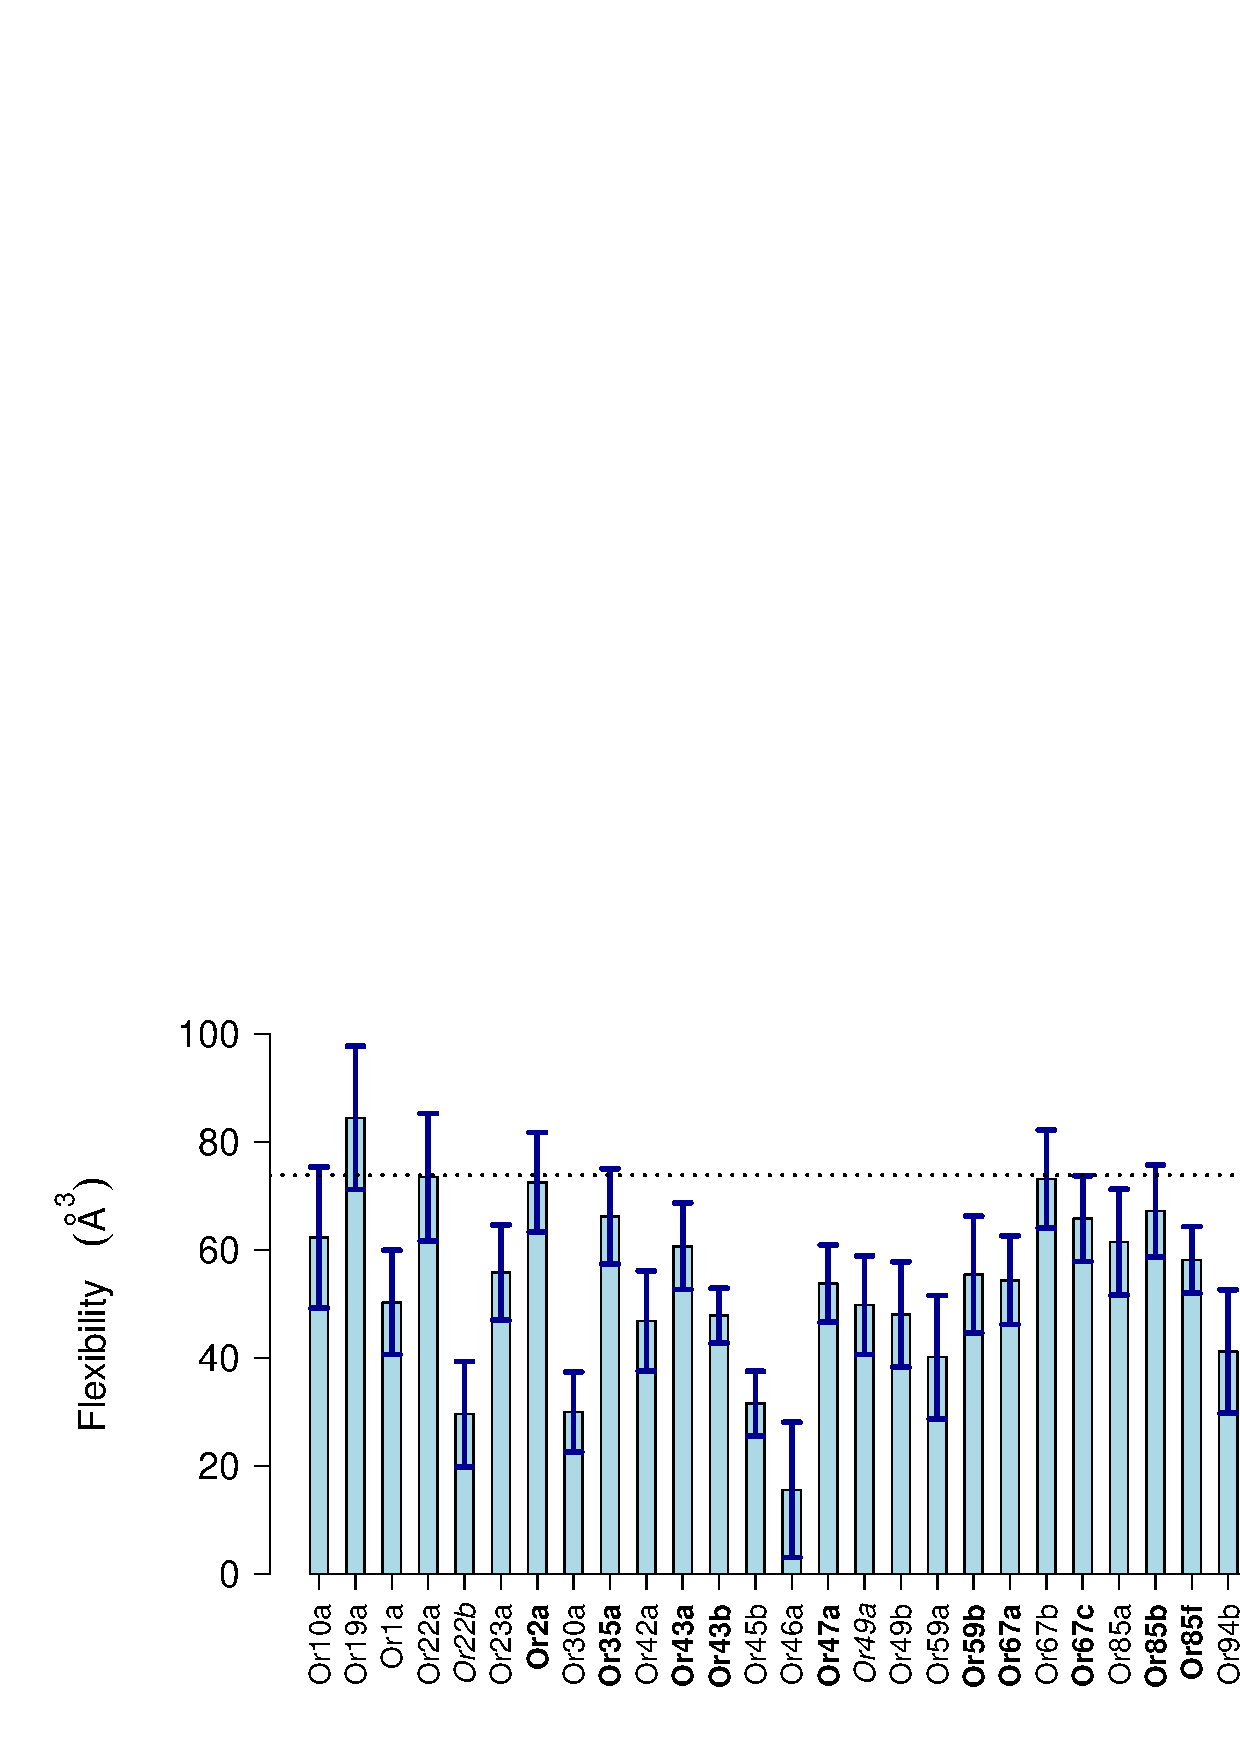
\includegraphics[width=\textwidth]{fig/std-vol}
\caption{std volume.}
\end{figure}•


\end{document}
